\chapter{Bitcoin Mining}

Recall that the \textbf{distributed consesus} is a procedure to reach a common agreement in a distributed or decentralized multi-agent system;
it must ensure correct results even in presence of faulty nodes, network partitioning and byzantine faults\footnote{Nodes behaving maliciously}.
\note{Even though it is difficult to classify the method used by Bitcoin to achieve decentralization from a theoretical point of view, it works in practice.

\textit{``...is not purely technical, but it's a combination of technical methods and clever incentive engineering.''}
}

\section{Competing}
Every node holds a \texttt{MemPool} containing all Bitcoin transactions awaiting confirmation.
Conflicts may happen there, not in the ledger.
In case a node receives a double-spending transaction, it will keep the first one and discard the second one.\\
Nodes try to get transactions into the ledger, and \textbf{compete} to do so.
Nakamoto consesus is implemented like a ``lottery'' where the winner gets to add a block ---of valid transactions--- to the blockchain, and to send its neighbours the updated ledger. The process of competing to add transactions to the blockchain is called \textbf{mining}.

\subsection{Mining}
Mining process starts with filling a candidate block with transactions taken
from the memory pool, and then building a block header (1000 times smaller than the block);
finally the node performs the Proof of Work.\\
So, while a single transaction may be built by anyone, blocks are built by miners, and include multiple transactions and the header.

The block header contains:
\begin{itemize}
   \item Version
   \item Timestamp
   \item \texttt{mhash} The Merkle root of the transactions in the block
   \note{Merkle tree is not explicitly represented in the block, it is built on demand}
   \item \texttt{hashprev} The hash of the previous block
   \item PoW related fields:
   \begin{itemize}
      \item Target
      \item Nonce
   \end{itemize}
\end{itemize}

\framedt{Mining}{
   \begin{enumerate}
      \item Set \texttt{nonce = 0}
      \item Hash the block header including the \texttt{nonce}
      \item \texttt{while (\texttt{hash} > \texttt{target})}
      \begin{enumerate}
         \item Increment \texttt{nonce}
         \item Hash the block header including the \texttt{nonce}
      \end{enumerate}
   \end{enumerate}
   Target acts as threshold, and represents the number of leading zeros the hash must have.
   The nonce is 32 bit long, and even a slight increment on it changes the whole hash result.
}

\subsection{Consesus}
Node is selected to propose the next block in proportion to a resource that it is hard to
monopolize: in Bitcoin this resource is \textbf{computational power} and the selection is done on the basis of the Proof of Work.

The Consensus is \textbf{implicit}:
\begin{itemize}
   \item No collective distributed algorithm executed by the nodes
   \item No voting
   \item Selection of malicious nodes is also implicitily handled by the system
\end{itemize}

Even if the nodes may have occasionally an inconsistent view of the ledger (blockchain forks) consensus will eventually occur, the consistent ledger will eventually be the longest chain.
\note{This is true if the majority of the nodes are honest.}

\subsection{Proof of Work}
\begin{itemize}
   \item \texttt{d} - \textit{difficulty}: a positive number which is used to adjust the time to execute the proof
   \item \texttt{c} - \textit{challange}: a given string (the block header minus the nonce)
   \item \texttt{x} - \textit{nonce}: an unknown string
\end{itemize}

\begin{definition}[Proof of Work]
   A proof of work is a function $F_d(c,x) \rightarrow {\texttt{True,False}}$ satisfying:
   \begin{enumerate}
      \item \texttt{d} and \texttt{c} are \textit{fixed}
      \item $F_d(c,x)$ is \textit{fast to compute}, if \texttt{d}, \texttt{c}, and \texttt{x} are known
      \item instead, finding \texttt{x} so that $F_d(c,x) = \texttt{True}$ is computationally difficult, but feasible.
   \end{enumerate}
\end{definition}

The PoW is hard to solve because the computing output looks like a random 256-bit string where each bit is equally likely to be \texttt{0} or \texttt{1} independently of the other bits, so each output bit looks like coin flips (\texttt{0/1}).
There is no better way of finding the correct output than trying by \textbf{brute force}.\\
The probability $p$ that the block hash is below the target $T$ and average number of attempts $a$ to find a solution are:
\begin{align*}
   p=\frac{T+1}{2^{256}} & & a=\frac{1}{p}
\end{align*}

The system is resistant to Sybil attacks because the PoW is a scarce resource, and the cost of the attack is proportional to the whole computational power of the attacker, not to the number of identities they have.

\note{The Proof of Work is also used in other contexts to prevent spam, like in Hashcash, and to counter DoS attacks, by allowing users to access a service only after solving a PoW.

Email spam may be prevented through a PoW by adding a post stamp to each email message, and the receiver may decide to accept the message only if the PoW is valid.}

\subsection{Block propagation and incentives}
\paragraph{Block propagation}
The mined block is broadcasted on the network, and each node receiving the block verifies that the PoW has been solved by hashing the block header and checking that the hash is less than the target.
It is easy to verify, without centralization points.\\
After the verification, the node adds the block to the blockchain and kicks out any conflicting transaction from \texttt{MemPool}.

\paragraph{Incentives}
There are two mechanisms to incentivize the miners to be honest:
\begin{enumerate}
   \item \textbf{Block reward}:
   a payment to the miner in exchange for the service of creating a block.\\
   Bitcoin mints new coins when a new block is mined, and is the only way to create new bitcoins.\\
   The reward is halved every 210K blocks ($\sim 4 \textit{ years}$), and the last block reward will be mined in 2140.
   \item \textbf{Transaction fees}:
   for each transaction in the block the miner gets the difference between transaction inputs and outputs.\\
   It was voluntarily inserted to obtain a good ``quality of service'' from the miners.
\end{enumerate}

The first transaction in each block is called \ul{\textbf{coinbase transaction}, and is the one that mints new coins}: it includes the reward plus the transaction fees to the miner, and is not linked to any previous UTXO, but to a single ``dummy'' input.

\framedt{Mining Difficulty}{
   \begin{center}
      \textit{``To compensate for increasing hardware speed and varying interest in running nodes over time, the proof-of-work difficulty is determined by a moving average targeting an average number of blocks per hour. If they're generated too fast, the difficulty increases.''}\\
      -Satoshi Nakamoto
   \end{center}
   The difficulty is adjusted every 2016 blocks (about 2 weeks) to keep the block time around \textbf{10 minutes}.
   The difficulty is adjusted by changing the target, which is inversely proportional to the difficulty.
}

\framedt{Why 10 Minutes?}{
   \begin{center}
      \textit{``If broadcasts turn out to be slower in practice than expected, the target time between blocks may have to be increased to avoid wasting resources. 
      We want blocks to usually propagate in much less time than it takes to generate them, otherwise nodes would spend too much time working on obsolete blocks.''}\\
      -Satoshi Nakamoto
   \end{center}

   The 10 minutes target time is a trade-off between the time to propagate a block and the time to generate a new one.\\
   The goal was to allow time to propagate across the whole network before the next block gets mined, to avoid wasting resources.
}

Note that 10 minutes mining time means that no instantaneous transactions are possible, but the system is designed to be secure, not fast.
\note{e.g. you can't pay for an ice cream using bitcoin.}

\begin{figure}[htbp]
   \centering
   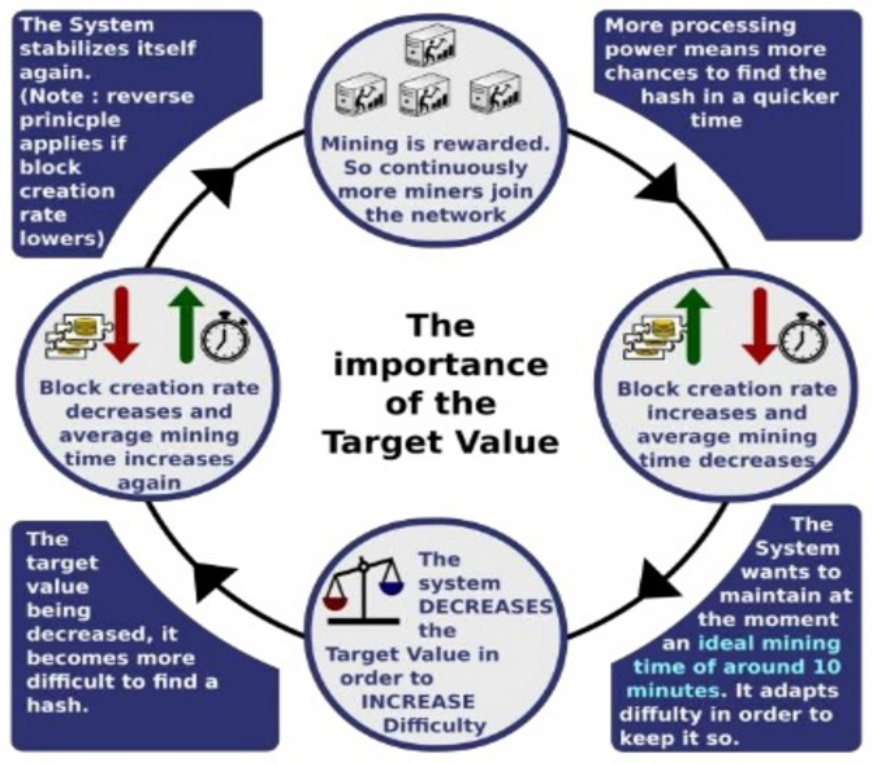
\includegraphics{images/bitcoin_targetcycle.png}
   \caption{Bitcoin target cycle}
   \label{fig:bitcoin_targetcycle}
   \note{A node can't avoid decreasing the target, since the other nodes would not validate its Proof of Work.}
\end{figure}

\note{Blocks are preferred over single transactions, because verification is faster and mining single transactions would overall require more mining work.}

\subsection{Tamper-freeness}
The blockchain is tamper-free because:
\begin{itemize}
   \item The PoW is hard to solve
   \item The PoW is easy to verify
   \item The PoW is a scarce resource
\end{itemize}

It would take an \ul{unfeasible amount of power for an attacker to change a transaction in a block}, since it would imply that: 
\begin{enumerate}
   \item The root of the Merkle tree changes and so the block header
   \item The nonce of the block is no more valid
   \item Re-execute PoW to re-compute the right nonce for the new block
   \item In the next block the hash pointer to the previous block changes as well
   \item Nonce of the next block is no more valid
   \item Need to re-execute also on next block...
   \item ...and so on
\end{enumerate}

\section{Temporary Forks}

\begin{paracol}{2}
   
   \colfill
   \ul{Temporary forks may happen when two miners find a valid block at the same time}, and broadcast it to the network.
   The state of the blockchain is seen by the nework consists of two branches both
   originating from the same parent block.
   In this case both branches are legitimate, and is different from the double spending case, but still, \textit{which bitcoin are really spent?}
   \colfill

   \switchcolumn

   \colfill
   \begin{figure}[htbp]
      \centering
      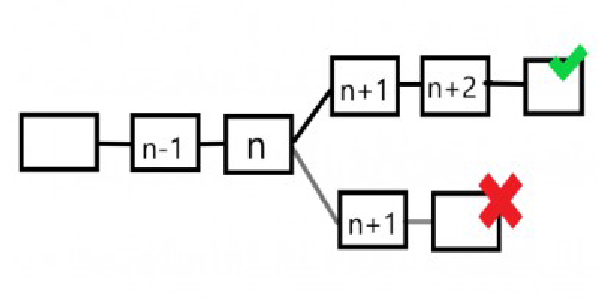
\includegraphics{images/bitcoin_forks.png}
      \caption{Bitcoin temporary forks}
      \label{fig:bitcoin_forks}
   \end{figure}
   \colfill
\end{paracol}
   

Each miner node either receives block A or block C first, which are both valid, but different,
and then starts mining on the branch of the fork with the block it received first;
note that the two forks may grow indipendently, and the network may have multiple branches.
If a \ul{miner receives a block that makes the other fork longer, it \textit{abandons} the
shorter fork};
the transactions of the ``abandoned'' fork that were not approved in the winning fork are returned to the pool of ``not-yet-approved'' transactions.
\begin{definition}[6 Confirmation Rule]
   Bitcoin approves a transaction finally only once there are at least \textbf{five} following blocks in the chain 
\end{definition}

\framedt{May the two chains extended perfectly in parallel, to equal height?}{
   It may be possible, but extremely unlikely in practice.
   The probability that this happens recursively, for a long period is very low,
   besides mining and the block propagation delay introduce randomness in the protocol that typically prevents this.

   Recall that each miner switches to mine on the longest branch it becomes aware of.
}

\begin{definition}[Nakamoto Consesus]
   Forks are \textit{eventually} resolved and all nodes eventually agree on which is the longest
   blockchain. The system therefore guarantees \textbf{eventual consistency}.
\end{definition}

\section{Mining technologies}
The main Bitcoin actors are:
\begin{enumerate}
   \item Reference client (Bitcoin Core)
   \item Full block chain mode
   \item Solo miner
   \item Lightweight (SPV) wallet
\end{enumerate}

Basically, the mining process is SHA computation which can be summarized as follows:
\begin{lstlisting}
   while (1)
      HDR[kNoncePos]++;
      if (SHA256(SHA256(HDR)) < (65535 << 208)/ DIFFICULTY)
         return;
\end{lstlisting}
To compute such hash, CPUs were initially used, then GPUs,GPU pools, FPGAs ---Verilog programmable hardware--- and now ASICs are used.
It is unclear what will ASICs successor be.
ASICs stands for Application Specific Integrated Circuits, and are hardware devices specifically designed to perform a task, e.g. mining.
For this task, they are faster and more efficient than CPUs and GPUs.

\subsection{Centralized Mining pools}
\ul{Mining is a very risky task}, since it is very likely to spend a lot for mining hardware and eletricity without
obtaining a reward for a long time.
\textbf{Mining pools} are a way to share the risk and the reward among the participants. 

The \textbf{Pool Manager} sends blocks to miners and distributes the reward among the participants, based on the work they have performed; it must be trusted by anyone.
\labelitemize{\textit{Challenges}}{
\begin{itemize}
   \item How does a pool manager know how much work each member of the pool is actually performing?
   \note{Also miners that have not been able to solve the PoW have to be rewarded for their work.}
   \item How can the pool manager divide the revenue proportional to the amount of work each miner is doing?
   \note{Partecipants to the pool may cheat claim that they've done more than they actually did.\\
   It is in general hard to prove how much work a node has performed. Generally some ``near-valid blocks'' are sent to the pool manager, to indicate that the miner is actually working.}
\end{itemize}   
}

\textit{Pay-per-share} (PPS) is a common reward system used by mining pools, where the pool manager pays a fixed amount for each share submitted by the miner.
Miner's are payed from pool's existing balance, and there is no special reward for the miner who actually mines the block.

\textit{Pay-proportional} is instead a reward system where the pool manager enacts a reward proportional to the amount of work done by the miner, making miners more incentivized to present valid blocks.
This is less riskful for the pool manager, since payment is enacted only when a block is mined.

\subsection{Decentralized Mining pools}
\begin{paracol}{2}
   
   The basic idea behind decentralized mining pools is to build a separate, private chain including \textit{``weak blocks''} mined with lower difficulty, store in the private chain called \textit{``sharechain''}transactions rewarding for mining weak blocks
   until a valid block is found;
   at that point reward is distributed through a side blockchain which is then merged to the main chain, hence obtaining a transparent and fair payout scheme with efficiency minimal performance overhead.

   \switchcolumn

   \begin{figure}[htbp]
      \centering
      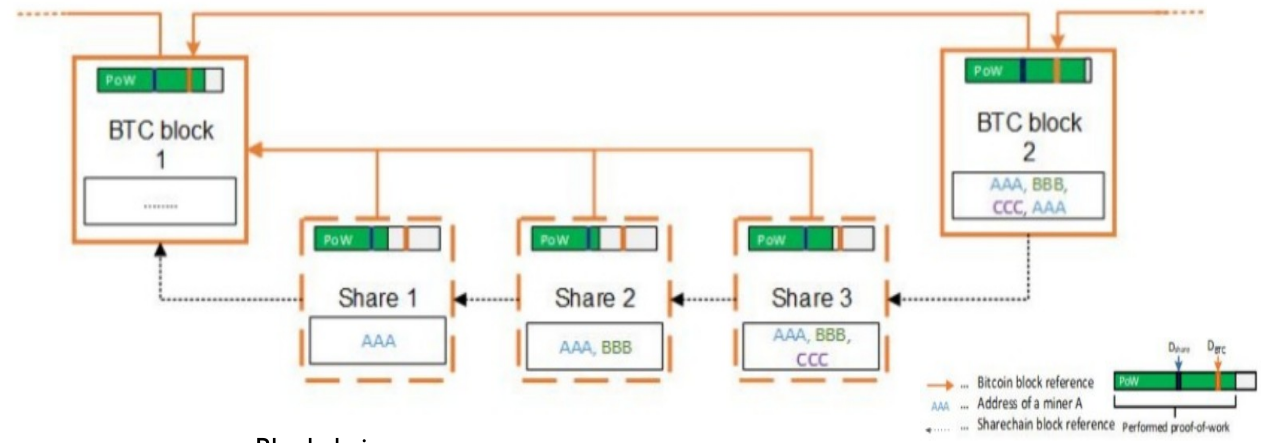
\includegraphics{images/bitcoin_decentralized_pool.png}
      \caption{Sharechain and main bitcoin chain}
      \label{fig:bitcoin_decentralized_pool}
   \end{figure}

\end{paracol}